\documentclass[12pt,a4paper]{article}

% -------------------
% MARK: Packages
% -------------------

% import geometry package to update the document margins
\usepackage[margin=1in]{geometry}
% set the font to helvectica
\usepackage[scaled]{helvet}
\renewcommand\familydefault{\sfdefault}
% for type-setting
\usepackage{amsmath, amssymb, amsfonts, verbatim, pifont}
% for slashed out text
\usepackage[normalem]{ulem}
% for units and scientific notation
\usepackage[table]{xcolor}
\usepackage{siunitx}
% for references and URLs
\usepackage{hyperref, url}
% Natbib setup for author-year style
\usepackage{natbib}
 \bibpunct[, ]{(}{)}{,}{a}{}{,}%
 \def\bibfont{\small}%
 \def\bibsep{\smallskipamount}%
 \def\bibhang{24pt}%
 \def\newblock{\ }%
 \def\BIBand{and}%
% for graphics and figures
\usepackage{graphicx, subfig, tikz}
% force figures to stay in their sections
\usepackage[section]{placeins}
% for tables
\usepackage{booktabs, longtable, tabularx}
\usepackage{multicol, multirow}
\usepackage{adjustbox}
\usepackage[flushleft]{threeparttable}
% a package for working with .csv data for tables
\usepackage{csvsimple}
% setup the algorithm package
% ruled: show bars around title and bar at bottom
% lined: show the line column on the left of the algorithm
% linesnumbered: print line numbers for each line
\usepackage[ruled,lined,linesnumbered]{algorithm2e}
\DontPrintSemicolon % don't print the semicolon that \; usually prints
% fix overfull hbox errors from oddities like using
% quotes (``foo'') and etc.
\usepackage{microtype}

% -------------------
% MARK: Debugging Packages
% -------------------

% import a debugging package to show the margin boxes
% \usepackage{showframe}

% -------------------
% MARK: Declarations
% -------------------

% setup captions for tables and figures
\captionsetup[table]{%
  labelfont={bf},
  name={Table},
  labelsep=colon,
  justification=raggedright,
  singlelinecheck=false}
\captionsetup[figure]{%
  labelfont={bf},
  name={Figure},
  labelsep=colon,
  justification=raggedright,
  singlelinecheck=false}
\captionsetup[algorithm2e]{%
  labelfont={bf},
  name={Figure},
  labelsep=colon,
  justification=raggedright,
  singlelinecheck=false}

% set the graphics path to the img directory
\graphicspath{{img/}}

% -----------------------------------------------------------------------------
% MARK: algorithm2e stuff
% -----------------------------------------------------------------------------

% params
% \SetKwInOut{Objects}{$\CKmatrix{O}$}
% \SetKwInOut{Weights}{$\CKvector{w}$}

% -------------------
% MARK: Headers
% -------------------

% headers and footers
\usepackage{fancyhdr}
\setlength{\headheight}{15pt}
\pagestyle{fancy}
\lhead{KautenjaDSP}
\rhead{\itshape SCC v1.5.0}
\cfoot{\thepage}

% start the document
\begin{document}

% -------------------
% MARK: Title Page
% -------------------

% fancyhdr directive to remove headers from this title page
\thispagestyle{empty}
% center the title page contents
\vspace*{\fill}
\begin{center}
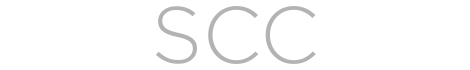
\includegraphics{SCC-Logo}
\linebreak\linebreak\linebreak\linebreak
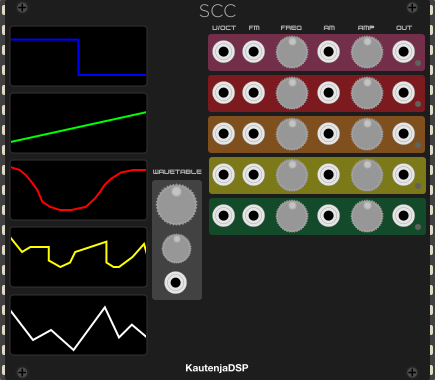
\includegraphics{SCC-Module}
\linebreak\linebreak\linebreak\linebreak

\includegraphics{KautenjaDSP}
\end{center}
\vspace*{\fill}
\clearpage

% -------------------
% MARK: Overview
% -------------------

\section{Overview}

% SCC is an emulation of the SCC sound chip from the Nintendo Entertainment System (NES) for VCV Rack. The SCC chip contains two pulse wave generators, a quantized triangle wave generator, and a noise generator. The original chip featured a DMC loader for playing samples that has been omitted in this emulation.

% SCC provides the key features of the SCC chip, namely,
% \begin{itemize}
%   \item \textbf{Dual pulse wave generator:} Dual 8-bit pulse waves with four duty cycles: $12.5\%$, $25\%$, $50\%$, and $75\%$;
%   \item \textbf{Quantized triangle wave generator:} Generate NES style triangle wave with 16 steps of quantization;
%   \item \textbf{Noise generator:} generate pseudo-random numbers at 16 different frequencies; and
%   \item \textbf{Linear Feedback Shift Register (LFSR):} for that old-school 8-bit randomness!
% \end{itemize}

% -------------------
% MARK: Panel Layout
% -------------------

\section{Panel Layout}

\begin{center}
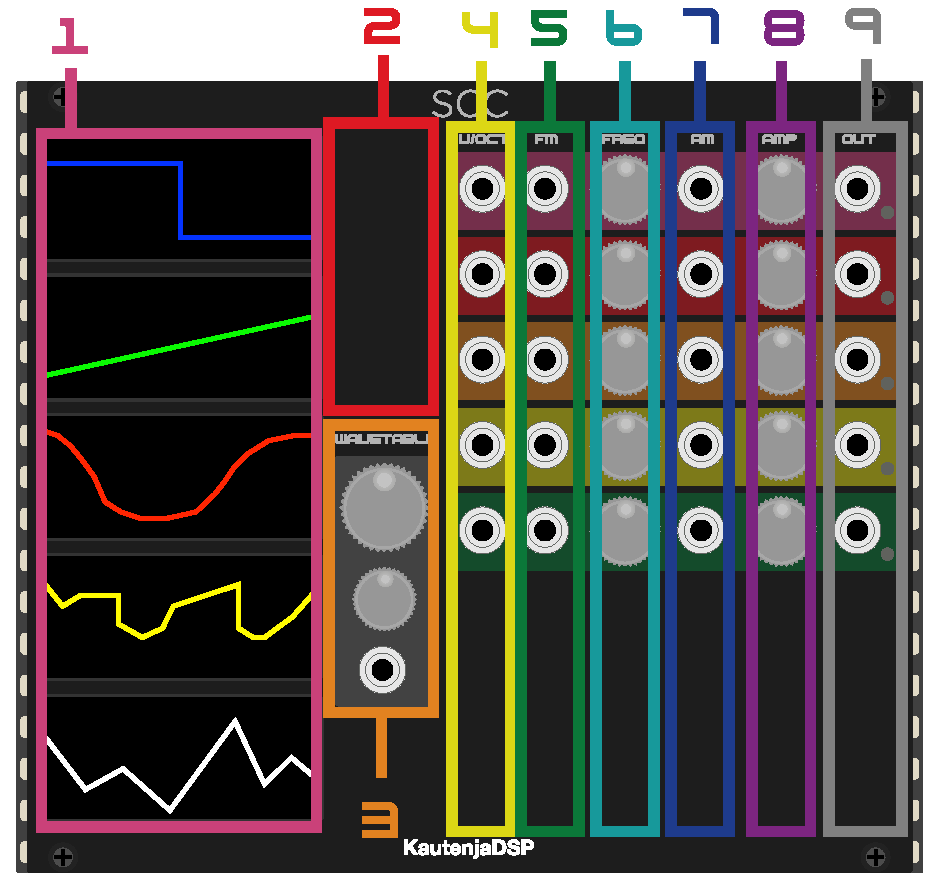
\includegraphics{SCC-Manual}
\end{center}

% \begin{enumerate}
%   \item Coarse frequency control over the four channels.
%   \item $V$/Octave inputs for pulse1, pulse2, and triangle waveform generators.
%   \item linear CV frequency modulation for pulse1, pulse2, and triangle waveform generators.
%   \item Pulse width selector. Chooses between four duty cycles: $12.5\%$, $25\%$, $50\%$, and $75\%$.
%   \item CV LFSR gate, high at $2V$. Holds the LFSR generator as long as the input voltage is $>2V$.
%   \item Period of randomness $\in [0, 15]$ for the noise generator. See \url{https://wiki.nesdev.com/w/index.php/APU_Noise} for approximate frequency and pitch mappings.
%   \item Channel outputs, ${\approx}10V_{pp}$.
% \end{enumerate}

% -------------------
% MARK: References
% -------------------

\clearpage
\renewcommand\refname{References \& Acknowledgments}
\nocite{*}
\bibliographystyle{apalike}
\bibliography{references}

\end{document}
